\chapter{Verification of sections relating to Ultimate and Serviceability Limit States}
\section{Verification of shell sections}
\subsection{Sections definition}
\subsubsection{hormigonesEHE}
\begin{verbatim}
from materials.ehe import hormigonesEHE
\end{verbatim}

\subsubsection{EHE\_reinforcing\_steel}
\begin{verbatim}
from materials.ehe import EHE_reinforcing_steel
\end{verbatim}

\subsubsection{RecordSeccionHALosa}
\begin{verbatim}
from materials.fiber_section import defSeccionHASimple
\end{verbatim}


\subsection{Types of calculation}
\subsubsection{defInteractionDiagram}

\subsubsection{simple\_static\_linear}
\begin{verbatim}
from solution import predefined_solutions
predefined_solutions.simple_static_linear
\end{verbatim}

\subsection{Limit State at Failure under normal stresses verification}

\subsubsection{lanzaCalculoTNFromXCData}
This function carries out the verification of the limit state at failure under nornal stresses. It takes as input the internal forces and bending moments calculated for the shell elements for every ULS combinations, the sections definition and the interaction diagrams to be employed.

The function returns two files with the verification results:
{\tt nmbArchSalida.py}: XC file that assigns each shell element the capacity factor (worst-case) {\tt FCC} calculated for reinforcement in directions 1 and 2, together with the concomitant axial force and bending moments {\tt NCP MyCP MzCP}.
{\tt nmbArchSalida.py}: \LaTeX\  file containing a table with the following items:

\begin{center}
\begin{tabular}{ccccccc}
\multicolumn{7}{l}{\textbf{Section 1}} \\
\\
Element & Section & ULS & Axial & Bending & Bending & Capacity \\
number  & name & name & force NCP1 & moment MyCP1 & moment MzCP1 & factor FCCP1 \\
\hline
\multicolumn{7}{l}{\ldots\ \ldots\ \ldots} \\
\\
\multicolumn{7}{l}{\textbf{Section 2}} \\
\\
Element & Section & ULS & Axial & Bending & Bending & Capacity \\
number  & name & name & force NCP2 & moment MyCP2 & moment MzCP2 & factor FCCP2 \\
\hline
\multicolumn{7}{l}{\ldots\ \ldots\ \ldots} \\
\\

\end{tabular}
\end{center}

\begin{figure}[h]
\centering
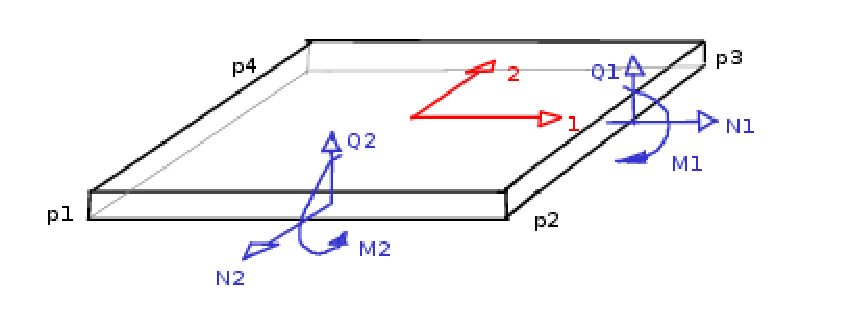
\includegraphics[width=100mm]{materials/figures/signosEsfuerzos}
\caption{Positive directions of forces and moments in shell elements}\label{shell_forces_moments}
\end{figure}

 
\begin{verbatim}
from materials.xLamina import calculo_tn
calculo_tn.lanzaCalculoTNFromXCData(mdlr,analysis,nmbArchCsv,nmbArchSalida, 
mapSectionsForEveryElement,mapSectionsDefinition, mapInteractionDiagrams)
\end{verbatim}
\begin{paramFuncTable}
\mdlr{} \\
\analysis{} \\
\nmbArchCsv{ULS under normal stresses}\\
\nmbArchSalida{}\\
\mapSectionsForEveryElement{} \\
\mapSectionsDefinition{} \\
\mapInteractionDiagrams{} \\
\end{paramFuncTable}


\subsection{Limit State of Failure due to shear verification}
\begin{verbatim}
from materials.xLamina import calculo_v
calculo_v.lanzaCalculoV(mdlr,analysis,nmbArchCsv,nmbArchSalida, 
mapSectionsForEveryElement,mapSectionsDefinition,mapInteractionDiagrams,
trataResultsCombV)
\end{verbatim}

\begin{paramFuncTable}
\mdlr{} \\
\analysis{} \\
\nmbArchCsv{ULS due to shear}\\
\nmbArchSalida{}\\
\mapSectionsForEveryElement{} \\
\mapSectionsDefinition{} \\
\mapInteractionDiagrams{} \\
\trataResultsCombV{} \\
\end{paramFuncTable}


\subsection{Cracking limit state verification}
\begin{verbatim}
from materials.xLamina import calculo_fis
calculo_fis.lanzaCalculoFISFromXCDataPlanB( )
\end{verbatim}
%\subsection{defMaterialesK}
%\noindent This function sets up the sections definition to be used for the verifications relating to Cracking Limit State. Characteristic values are used to define the properties of the materials (concrete, reinforcing steel) that make up the section.
%\begin{verbatim}
%from materials import xLamina
%xLamina.defMateriales.defMaterialesK(mdlr,path, nmbScc1, nmbScc2)
%\end{verbatim}
%\begin{paramFuncTable}
%\mdlr{} \\
%{\tt defSecc} &   name identifying the class object used to define the properties of the section.\\
%\end{paramFuncTable}







\section{Verification of beam sections}

